%%%%%%%%%%%%%%%%%%%%%%%%%%%%%%%%%%%%%%%%%
% Memo
% LaTeX Template
% Version 1.0 (30/12/13)
%
% This template has been downloaded from:
% http://www.LaTeXTemplates.com
%
% Original author:
% Rob Oakes (http://www.oak-tree.us) with modifications by:
% Vel (vel@latextemplates.com)
%
% License:
% CC BY-NC-SA 3.0 (http://creativecommons.org/licenses/by-nc-sa/3.0/)
%
%%%%%%%%%%%%%%%%%%%%%%%%%%%%%%%%%%%%%%%%%

\documentclass[letterpaper,11pt]{texMemo} % Set the paper size (letterpaper, a4paper, etc) and font size (10pt, 11pt or 12pt)

\usepackage{parskip} % Adds spacing between paragraphs
\usepackage[colorlinks]{hyperref}
\usepackage{graphicx}
\usepackage{float}
\usepackage{listings}
\hypersetup{citecolor=DeepPink4}
\hypersetup{linkcolor=red}
\hypersetup{urlcolor=blue}
\usepackage{cleveref}
\setlength{\parindent}{15pt} % Indent paragraphs

%----------------------------------------------------------------------------------------
%	MEMO INFORMATION
%----------------------------------------------------------------------------------------

%----------------------------------------------------------------------------------------
%	MEMO INFORMATION
%----------------------------------------------------------------------------------------

\memoto{Dr.Jeff McGough} % Recipient(s)

\memofrom{Benjamin Lebrun} % Sender(s)

\memosubject{Homework 3} % Memo subject

\memodate{\today} % Date, set to \today for automatically printing todays date

%\logo{\includegraphics[width=0.1\textwidth]{logo.png}} % Institution logo at the top right of the memo, comment out this line for no logo

%----------------------------------------------------------------------------------------

\begin{document}


\maketitle % Print the memo header information

%----------------------------------------------------------------------------------------
%	MEMO CONTENT
%----------------------------------------------------------------------------------------

\section*{Problem 3.4}
\subsection*{Problem statement}
Assume that you have a rectangular Mechanum robot with $L_1=0.30$m, $L_2=0.20$m and $r=0.08$m. Find the path of the robot
for the given wheel rotations: $\dot{\phi}_1 = 0.75*\cos(t/3.0)$, $\dot{\phi}_2 = 1.5*cos(t/3.0)$, $\dot{\phi}_3 = -1.0$, $\dot{\phi}_4 = 0.5$.
Start with $x, y, \theta = 0$ and set $t=0$, $\Delta t = 0.05$. Run the simulation for 200 iterations (or for 10 seconds).
Keeping the x and y locations in an array is an easy way to generate a plot of the robot’s path. If x, y are arrays of x-y
locations then try

\begin{tiny}
    \begin{lstlisting}
    import pylab as plt
    plt.plot(x,y,'b.')
    plt.show()
    \end{lstlisting}
\end{tiny}

Showing the orientation takes a bit more work. Matplotlib provides a vector plotting method. You need to hand it the location
of the vector and the vector to be plotted, $(x,y,u,v)$, where $(x,y)$s the vector location and $(u,v)$ are the x and y
components of the vector. You can extract those from $\theta$ using $u = s*\cos(\theta)$ and $v = s*\sin(\theta)$ where
$s$ is a scale factor (to give a good length for the image, e.g. 0.075). The vector plot commands are then

\begin{tiny}
    \begin{lstlisting}
    plt.quiver(u,v,c,s,scale=1.25,units='xy',color='g')
    plt.savefig('mecanumpath.pdf')
    plt.show()
    \end{lstlisting}
\end{tiny}

\subsection*{Solution approach and algorithm description.}
This problem required the use of the forward kinematic equations for mecanum drive robots.
Found in the book we simply use the equations

\[
    \dot{x}=\frac{r\Delta t}{4} A\cos(\theta_{k})  - B \sin(\theta_{k}
\]

\[
    \dot{y}=\frac{r\Delta t}{4} A\sin(\theta_{k})  + B \cos(\theta_{k})
\]

\[
    \dot{\theta}= \frac{r\Delta t}{4} \frac{1}{(L_1+L_2) } C
\]

where

\[A = \left(\dot{\phi}_{FL} + \dot{\phi}_{FR} + \dot{\phi}_{BL} + \dot{\phi}_{BR}\right)\]
\[B = \left( -\dot{\phi}_{FL} + \dot{\phi}_{FR} + \dot{\phi}_{BL} - \dot{\phi}_{BR}\right)\]
\[C = \left( -\dot{\phi}_{FL} + \dot{\phi}_{FR} - \dot{\phi}_{BL} +\dot{\phi}_{BR} \right)\]

Given our $\phi$ values of $\dot{\phi}_1 = 0.75*\cos(t/3.0)$, $\dot{\phi}_2 = 1.5*cos(t/3.0)$,
 $\dot{\phi}_3 = -1.0$, and $\dot{\phi}_4 = 0.5$, we write equations for the $A$, $B$, and $C$ equations,
 then feed these results into the $\dot{x}$, $\dot{y}$, and $\dot{\theta}$ equations.

\begin{figure}[ht]
\caption{Graphed path of Robot}
\centering
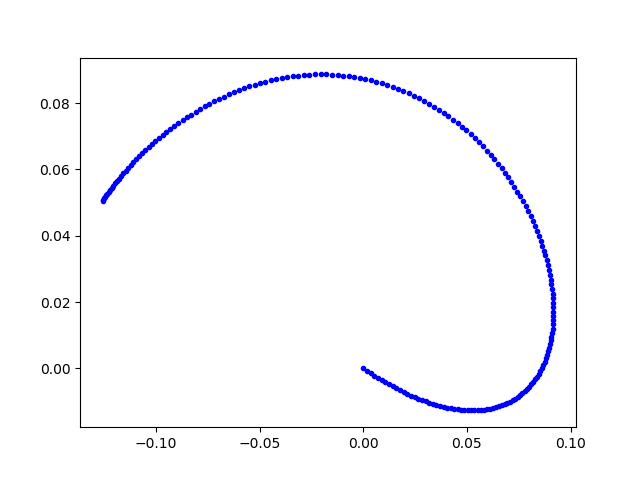
\includegraphics[scale=0.45]{img/P4a.png}
\end{figure}

\begin{figure}[ht]
\caption{Graphed path and orientation of Robot}
\centering
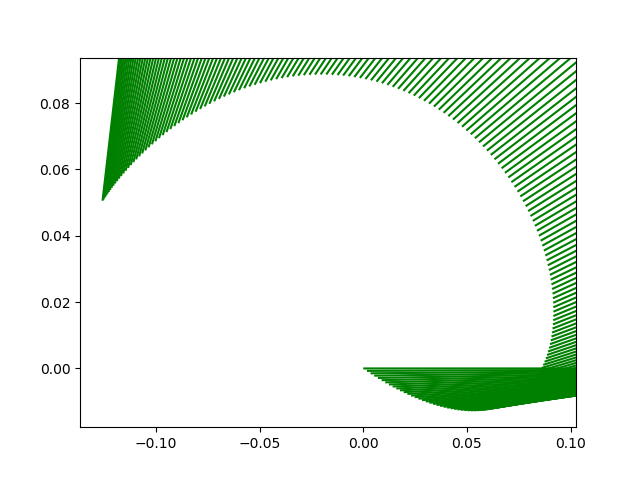
\includegraphics[scale=0.45]{img/P4b.png}
\end{figure}

\newpage
\subsection*{Code for Problem 4}
\begin{tiny}
\lstinputlisting{../P4.py}
\end{tiny}

\newpage
\section*{Problem 3.5}
\subsection*{Problem statement}
Real motion and measurement involves error and this problem will introduce the concepts.
Assume that you have a differential drive robot with wheels that are 20cm in radius and 
L is 12cm. Using the differential drive code (forward kinematics) from the text, develop 
code to simulate the robot motion when the wheel velocities are $\dot{\phi}_1 = 0.25t^2$,
$\dot{\phi}_2 = 0.5t$. The starting location is [0,0] with $\theta = 0$.

a. Plot the path of the robot on $0 \leq t \leq 5$. It should end up somewhere near [50,60].

b. Assume that you have Gaussian noise added to the omegas each time you evaluate the velocity
(each time step). Test with $\mu = 0$ and $\sigma = 0.3$. Write the final location (x,y) to a 
file and repeat for 100 simulations. Hint:

\begin{tiny}
    \begin{lstlisting}
        mu, sigma = 0.0, 0.3
        xerr = np.random.normal(mu,sigma, NumP)
        yerr = np.random.normal(mu,sigma, NumP)
    \end{lstlisting}
\end{tiny}

c. Generate a plot that includes the noise free robot path and the final locations for the
simulations with noise. Hint:

\begin{tiny}
    \begin{lstlisting}
        import numpy as np
        import pylab as plt
        ...
        plt.plot(xpath,ypath, 'b-', x,y, 'r.')
        plt.xlim(-10, 90)
        plt.ylim(-20, 80)
        plt.show()
    \end{lstlisting}
\end{tiny}

d. Find the location means and 2x2 covariance matrix for this data set, and compute the eigenvalues
and eigenvectors of the matrix. Find the ellipse that these generate. [The major and minor axes
directions are given by the eigenvectors. Show the point cloud of final locations and the ellipse 
in a graphic (plot the data and the ellipse). Hint:

\begin{tiny}
    \begin{lstlisting}
        from scipy import linalg
        from matplotlib.patches import Ellipse
        s = 2.447651936039926
        #  assume final locations are in x & y
        mat = np.array([x,y])
        #  find covariance matrix
        cmat = np.cov(mat)
        # compute eigenvals and eigenvects of covariance
        eval, evec = linalg.eigh(cmat)
        r1 = 2*s*sqrt(evals[0])
        r2 = 2*s*sqrt(evals[1])
        #  find ellipse rotation angle
        angle = 180*atan2(evec[0,1],evec[0,0])/np.pi
        # create ellipse
        ell = Ellipse((np.mean(x),np.mean(y)),r1,r2,angle)
        #  make the ellipse subplot
        a = plt.subplot(111, aspect='equal')
        ell.set_alpha(0.1)    #  make the ellipse lighter
        a.add_artist(ell)   #  add this to the plot
    \end{lstlisting}
\end{tiny}

\subsection*{Solution approach and algorithm description.}
For these graphs, we used the code included in section 3.1 of the text to create the relevant
datapoints for a differential drive robot. The points were then given a variance of error and the 
error added to the path of the robot to create a rought sketch of simulation. Then using the generation 
code for path points and error, a simulation file was created. This file can be viewed at 

\newpage
\subsection*{Code for Problem 5}
\begin{tiny}
\lstinputlisting{../P5.py}
\end{tiny}

\newpage
\section*{Problem 7.5}
\subsection*{Problem statement}
Can you think of a circuit to accept DC power which could hook up to the batteries either way.
[Meaning that if the user hooks up the wires backwards, it automatically still works].

\subsection*{Solution approach and algorithm description.}
The implementation of a full bridge recitfier would solve this issue. A full bridge rectifier is used 
in AC circuits to attempt to create a DC signal from an AC source. Implementing this with a DC battery is a 
trivial matter which should allow a battery to be inserted in any direction as a source, as shown below with some 
voltage drop across the diodes.

\begin{figure}[ht]
    \caption{Diagram of full bridge rectifier}
    \centering
    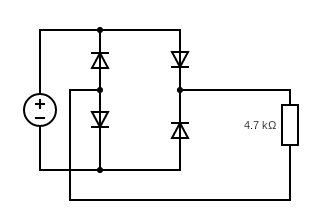
\includegraphics[scale=0.45]{img/FBR.png}
\end{figure}


\newpage
\section*{Problem 7.6}
\subsection*{Problem statement}
In an H bridge, are there switch combinations that cause problems? Why or why not?

\subsection*{Solution approach and algorithm description.}
Referencing figure 4, in an H bridge you should never close the Q1 and Q2 
circuits at the same time, or the Q3 or Q4. When this occurs, it's called "shoot through",
and may damage the circuit without proper protection (diodes, or dedicated protection circuit) 
at these bridges, especially if the main rail is a higher rated voltage than the  
two transistor/FET devices are rated for.

\begin{figure}[ht]
    \caption{Diagram of H bridge circuit}
    \centering
    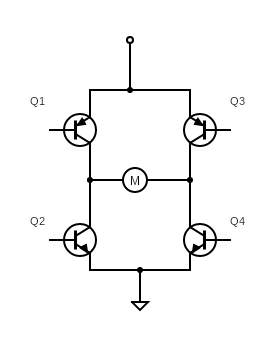
\includegraphics[scale=0.45]{img/Hbridge.png}
\end{figure}

\end{document}